\chapter{Discussions and Future Work}
\label{ch:discussion}
The overarching goal of this dissertation is to utilize the capability of a model checker to provide information that can be used during the safety analysis process. We leveraged the model checker to provide behavioral propagation of errors throughout nominal model contracts, we leveraged MIVC generation to provide compositional minimal cut set generation, and we use the counterexample generation capability to gain insight into the state of a system when a property is violated. All of this can be used within the iterative process of complex system design and development to show safety of a system and to drive for design change (see Section~\ref{subsec:mbsa}). We discuss in this chapter other ways of providing the analyst with safety critical information regarding model elements that may be of interest. 

\section{Graphical Fault Trees}
A typical fault tree generated by many of the current research tools available shows very little hierarchical information. An example of a flat fault tree is shown in Figure~\ref{fig:flatFT} and shows only the minimal cut sets that contribute to the top level event (TLE). 
\begin{figure}[h!]
	\centering
	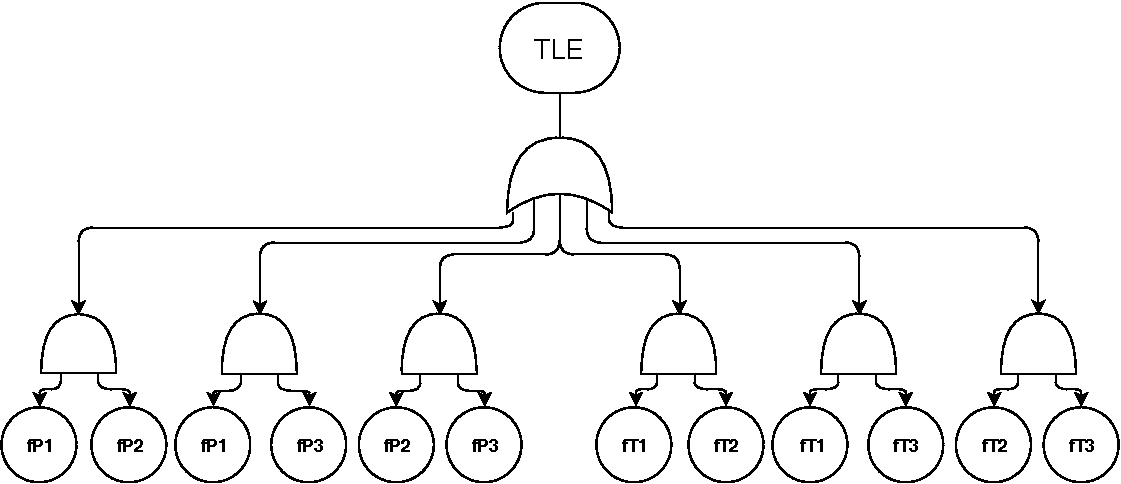
\includegraphics[trim=0 0 0 0,clip,width=0.8\textwidth]{images/flatFT.pdf}
	\caption{Flat Fault Tree for a Sensor Example}
	\label{fig:flatFT}
\end{figure}

The result of computing the minimal cut sets and presenting them in a tree-like structure was similar to this: a very short tree (one layer) with many branches. In essence, this provides no further information than that of a textual representation of the minimal cut sets. The nature of our minimal cut set generation approach is that the proofs are performed compositionally; this gives information regarding each level of analysis {\em per} each layer of architecture. This information can be used and printed out in a fault tree-like structure and, depending on the model, may provide the links between an active fault and the supporting guarantees it violates. An example of a hierarchical fault tree that could be produced by the information gathered through the minimal cut set algorithms defined in Chapter~\ref{chap:mcsGen} is shown in Figure~\ref{fig:ftSensor}. 

\begin{figure}[h!]
	\centering
	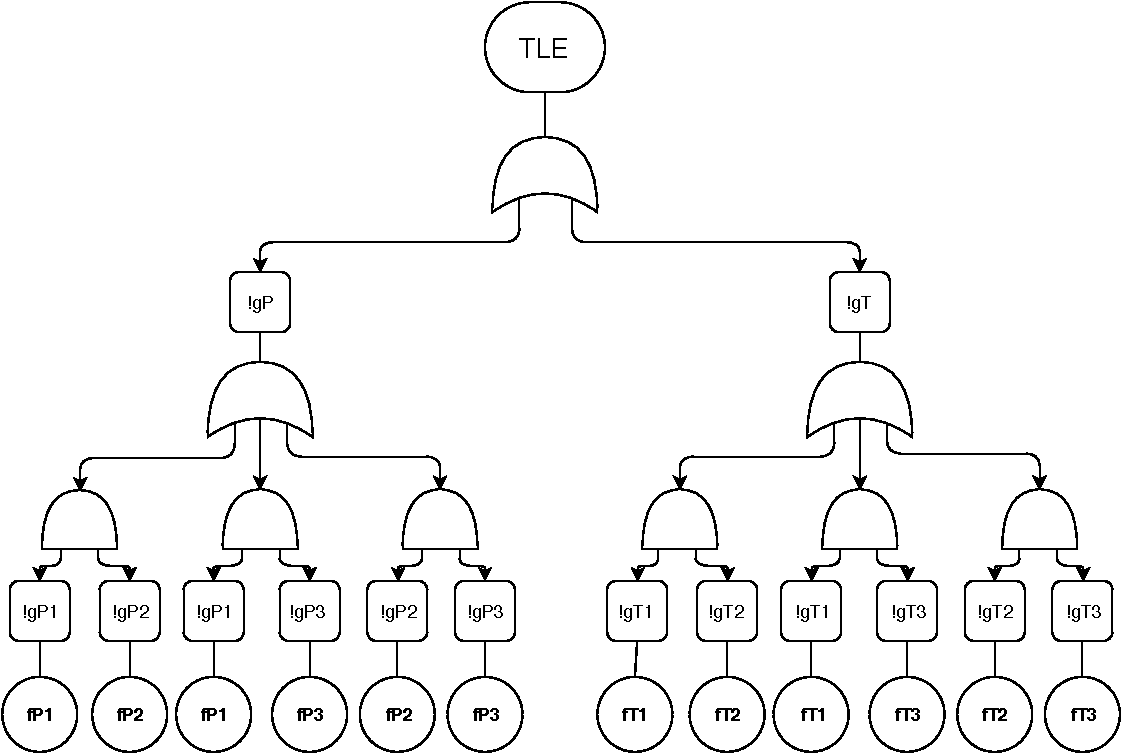
\includegraphics[trim=0 0 0 0,clip,width=0.8\textwidth]{images/ftSensor.pdf}
	\caption{Hierarchical Fault Tree for a Sensor Example}
	\label{fig:ftSensor}
\end{figure}

Each layer of the architecture is shown in the fault tree and represented by the violated contracts of that layer. The OR-gate between the lower level contracts and the top level event (violation of the safety property) reflects the property nicely: if either of the subsystems fail, the safety property is violated. The second layer of the tree also reflects the relationship between the sensors and the sensor subsystem: if any pairwise combination of sensors fail, the mid-level contract is violated. This process of using MIVCs to generate minimal cut sets will provide layer by layer the necessary information to not only collect the minimal cut sets, but also reflect the hierarchical nature of the system within the fault trees generated.

Upon initial exploration of the idea, two problems became apparent: (1) this relies on architectural depth of the model and provides no additional information if the architecture is a single layer, and (2) safety analysts wish to see fault trees as a kind of signal flow diagram and require a trace in signal from the error to the property violation. While our initial idea could partially address both issues, we began to look into a different method of analysis that may be able to address both issues. 

It became quickly apparent that to include in the analysis results information regarding the roles that faults, components, and node inputs play within a proof would provide great feedback to an analyst. They could view minimal cut sets from the perspective of the entire model and not just the faults that are active. If, for instance, certain components play direct roles in the proof of a safety property, those components would be seen as critical and managed or analyzed in a more comprehensive way. Likewise if specific inputs were known to be crucial to a proof, they would also be critical within the safety analysis. Preliminary investigations showed that related work may be used and extended to perform this kind of analysis~\cite{9081652}. 

\section{Compositional Probabilistic Analysis}
Safety analysis techniques aim at demonstrating that the system meets the requirements necessary for certification and use in the presence of faults. In many domains, there are two main steps to this process: (1) the generation of all minimal cut sets, and (2) the computation of the corresponding fault probability, i.e., the probability of violating the safety property given probabilities for all faults in the system. 

The probability of the Top Level Event (TLE), or violation of the safety property, is used to find the likelihood of the safety hazard that it represents. While evaluation of the fault model with a given probabilistic threshold does provide information on the safety hazards, it is also informative and desirable to find the overall probability of the occurrence of a hazard. 

Such computations can be carried out by leveraging the logical formula represented by the disjunction of all minimal cut sets which are in turn conjunctions of their constituents. 

Given a set of minimal cut sets and a mapping $\mathcal{P}$ that gives the probability of the basic faults in the system $f_i$, it is possible to compute the probability of occurrence of the TLE. Assuming that the basic faults are independent, the probability of a single minimal cut set, $\sigma$ is given by the product of the probabilities of its basic faults:
\begin{center}
    \begin{equation*}\mathcal{P}(\sigma) = \prod_{f_i \in \sigma} \mathcal{P}(f_i) 
    \end{equation*}    
\end{center}

For a set of minimal cut set, $S$, the probability can be computed using the following recursive formula:

\begin{center}
    $\mathcal{P}(S_1 \cup S_2) = \mathcal{P}(S_1) + \mathcal{P}(S_2) - \mathcal{P}(S_1 \cap S_2)$
\end{center}

Due to the independence assumption, $\mathcal{P}(S_1 \cap S_2)$ is computed as $\mathcal{P}(S_1) \cdot   \mathcal{P}(S_2)$. Using this technique, it is theoretically possible to compute the overall probability of a TLE given all minimal cut sets and an independence assumption, but in the real world of safety analysis this poses some problems, the largest of which is scalability. Given a very large system with many possible faults, it becomes difficult to compute all minimal cut sets without pruning of any kind. If one is unable to complete such computations, it is not possible to simply compute the probabilities as described above. 

As previously discussed, it is standard practice to consider cut sets only up to a given cardinality. As the cardinality of the cut sets increase, the likelihood of their occurrence decreases and as the system increases in size, the possible combinations of problematic faults will inevitably increase, at times exponentially. In order to simplify these calculations and address the problem of scalability, minimal cut sets up to a certain cardinality are considered. Everything above that is ``safely" ignored, and then specific criteria is used to over-approximate the error. The end result of these computations is above the actual probability (i.e., a safe approximation), but close enough to be significant. 

Another drawback to computing an exact probability of the TLE is the problem of model reliability and exactness; this corresponds exactly to the issue of granularity discussed in Chapter~\ref{chap:granularity}. For instance, if two groups of engineers each built a model of the same system, the models may not be equivalent; especially in terms of behavioral properties. Since our approach of computing minimal cut sets depends on the properties over system components, the calculated top-level probability will change. Different representations of the system will alter the computations.  

As an example, assume that Figure~\ref{fig:probComp1} is a snapshot of a given layer in a system designed by the first group of engineers. Component A has a contract, $G_A$, which is determined by the \aivcalg algorithm to depend on a lower level contract, $g_A = a \land b$. $g_A$ will be in the set of \textit{IVC}s for the contract $G_A$. Assume that only $a$ is required for the proof of $G_A$. 

\begin{figure}[h]
\begin{center}
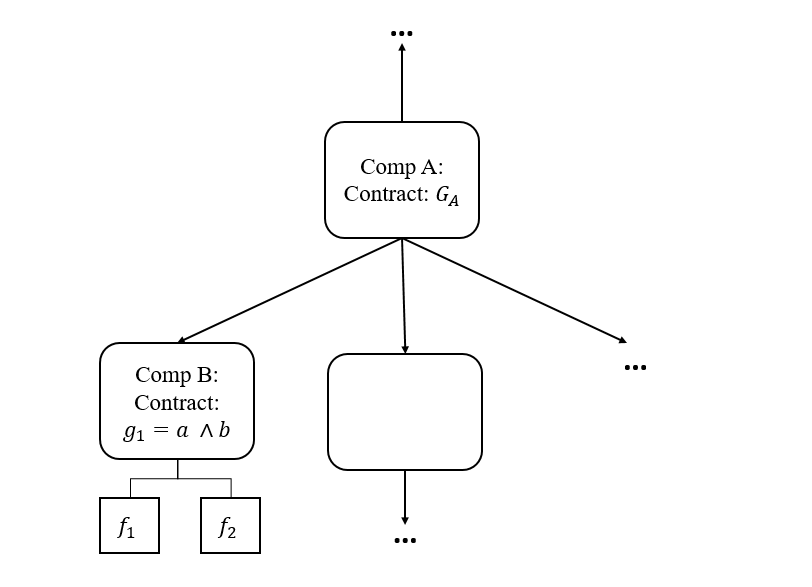
\includegraphics[width=6cm]{images/probComp1.PNG}
\caption{Sample System Contract Part I} \label{fig:probComp1}
\end{center}
\end{figure}

Two faults are defined on component B: $f_1$ violates $a$ and $f_2$ violates $b$. Since each of these faults will violate the contract $g_A$, each of these faults will be found in minimal cut set for $G_A$.

Now assume that Figure~\ref{fig:probComp2} was the system representation built by the second group of engineers. 
\begin{figure}[h]
\begin{center}
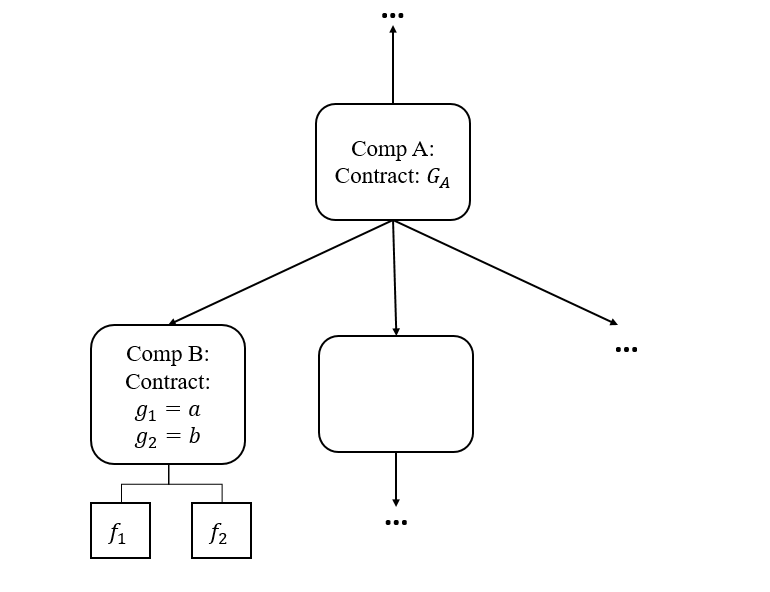
\includegraphics[width=6cm]{images/probComp2.PNG}
\caption{Sample System Contract Part II} \label{fig:probComp2}
\end{center}
\end{figure} 
The basic system structure is the same, but this time there are two contracts for component B: $g_1 = a$ and $g_2 = b$. Since $b$ is not required for the proof of $G_A$, only $g_1$ is found in the \textit{IVC}s for $G_A$ and thus only $f_1$ will be seen in the minimal cut sets for this particular contract. 

In this simple example, it is easy to see why a single computation of the top-level probability of a system may be misleading and may not reflect the actual probability of the system. To this end, we wish to find a way to accurately obtain higher and lower bounds of what the probability is likely to be. 

A lower bound for the probability can be obtained by choosing a maximum cardinality for each minimal cut set before computations begin, e.g. assume that cardinalities above $n$ are too unlikely to be significant. This will contribute to better scalability in large systems with numerous possible cut sets. A higher bound is commonly assigned by experts of the system, e.g. around 3 orders of magnitude higher than the lower approximation. 

It would be beneficial to leverage the  MIVC information to provide both the lower and upper bound approximations and show that these values are significant and trustworthy. 

\subsection{Mutations and Equation Removers}
\label{sec:granularityMutationEq}
For the development of model-based critical systems, it has been argued that formal proof should be applied to gain higher confidence in the model than with testing alone, e.g.~\cite{hardin2009development,miller2010software,rushby2009software,bozzano2003improving}. This has proven to be an active area of research, but has also shown some missing pieces -- one of which will be of benefit to us in this granularity exploration. When a property is proved valid, no further information is provided about the coverage of the model. One does not know whether the model contains features that are not covered by the properties~\cite{NFM2020Todorov}. Furthermore, we do not know if features \emph{within an IVC element in an MIVC set} are completely covered by the property. To this end, we began to look into mutation coverage to provide an answer. 

A mutation approach described by Todorov et al.~\cite{NFM2020Todorov} consists in mutating a model for which safety properties were proved valid, and trying to prove the same properties on the mutated models (\emph{mutants}). If the mutant is proved to be valid (i.e., it \emph{survived}), the mutant reveals part of the model that is not covered by the properties. We know that portion of the model is not necessary to find a proof. The approach described in this section attempts to use this type of mutant analysis on the contracts of a Lustre model, and thus compare to a granular refinement MIVC approach. 

A brief review of transition systems and some definitions are provided for convenience. 

Given a state space $U$, a transition system $(I,T)$ consists of an
initial state predicate $I : U \to \bool$ and a transition step
predicate $T : U \times U \to \bool$.
We define the notion of
reachability for $(I, T)$ as the smallest predicate $\reach : U \to
\bool$ which satisfies the following formulas:
\begin{gather*}
  \forall u.~ I(u) \Rightarrow \reach(u) \\
  \forall u, u'.~ \reach(u) \land T(u, u') \Rightarrow \reach(u')
\end{gather*}
A safety property $P : U \to \bool$ is a state predicate. A safety
property $P$ holds on a transition system $(I, T)$ if it holds on all
reachable states, i.e., $\forall u.~ \reach(u) \Rightarrow P(u)$,
written as $\reach \Rightarrow P$ for short. When this is the case, we
write $(I, T)\vdash P$.

The Lustre model is a set of equations$\{eq_1, \dots,eq_n\}$ and the transition relation $T$ has the structure of being a top level conjunction $T = t_1 \land \cdots \land t_n$ where each $t_i$ is an equality corresponding to $eq_i$. By further abuse of notation, $T$ is identified with the set of its top-level equalities. When an equation is removed from the Lustre model, an equality $t_i$ is removed from $T$ and the transition relation becomes $T\setminus \{t_i\}$. 

\begin{definition}
Minimal Inductive Validity Core (MIVC)~\cite{Ghassabani2017EfficientGO}: $S \subseteq T$ is a minimal Inductive Validity Core, denoted by $MIVC(P,S)$, iff $IVC(P,S) \land \forall T_i \in S$. $(I, S \setminus \{T_i\}) \not \vdash P$.
\end{definition}

In this research, we are only interested in minimal sets that satisfy a property $P$; if $(I, T) \vdash P$, then we know $P$ always has at least one MIVC which is not necessarily unique. By computing all MIVCs, we have a complete mapping from the requirements to the design elements; this is called \emph{complete traceability}~\cite{murugesan2016complete}. 

Ghassabani defines two metrics of coverage~\cite{ghassabani2017proof}. 

\begin{definition} \maycov\ : $t \in T$ is covered by $P$ iff $t_i \in $\maycov$(P)$, where \maycov$(P) = \{t_i | \exists S \in AIVC(P) \cdot t_i \in S\}$.
\end{definition}

\begin{definition} \mustcov\ : $t \in T$ is covered by $P$ iff $t_i \in $\maycov$(P)$, where \maycov$(P) = \{t_i | \forall S \in AIVC(P) \cdot t_i \in S\}$.
\end{definition}

The \maycov\ elements are relevant to the proof, but may be modified without affecting the satisfaction of $P$, whereas the \mustcov\ elements are absolutely necessary for the proof of $P$. One can view the \mustcov\ set of elements as the intersection of all MIVCs; if a single \mustcov\ element is removed, it ``breaks" all proofs of $P$. 

A mutator is formally a function that mutates any transition predicate $T$ to a set of mutants $\{T^1_{mut}, \dots, T^m_{mut}\}$, where each mutant $T^i_{mut}$ is obtained by applying a change to $T$. A very simple mutator is one that simply removes an equality $t_i$ from $T$, which amounts to removing the corresponding line of code from the Lustre model~\cite{NFM2020Todorov}. Todorov et al.~\cite{NFM2020Todorov} implemented an \emph{equation remover} in JKind which removes equations one by one and replays the proof process in an incremental way. If after removing an equation, the properties are still proved (the mutant survives), it means that the removed equation has no impact on the proof. If the properties do not hold any longer (the mutant is killed), then we know the removed equation is essential for the proof. This mutator computes the minimum \mustcov\ core. 


\subsection{Mutations and Guarantees}
\label{sec:granularityMutationInputs}
In the early stages of safety analysis on a complex critical system, it is beneficial to see what model elements may contribute to a property violation. While it is true that analysts will define faults based on their knowledge of the domain, at times in complex systems not all of these faults and their consequences are clear. Using the idea of mutations, we wish to see what the critical inputs to a system may be. 

As an example, we look once again at the sensor subsystem of a PWR as outlined in Chapter~\ref{chap:mcsGen}. Given a nominal system model containing the sensor subsystem and a single temperature sensor, we wish to see what model elements -- specifically guarantees -- are the \mustcov\  elements for the program. This tells the analyst that if these guarantees are violated, there are no paths to a proof of the property. 

To this end, we modified the equation remover implemented by Todorov, et al.~\cite{NFM2020Todorov} in JKind in order to collect killed guarantees from the program in Lustre. The analysis was run on a version of the sensor system with two subsystem guarantees: 

\begin{gather*}
\mathit{(env\_temp > 800) = high\_temp\_indicator}\\
\mathit{env\_temp = temp\_reading}
\end{gather*}

and one top level property:
\begin{gather*}
\mathit{(env\_temp > 800) = temp\_sensor\_high}\\
\end{gather*}

It is easy to see that a single subsystem level guarantee is sufficient to prove the property. The results from the modified equation remover shows the following guarantee that is critical to any proof of the safety property (Figure~\ref{fig:guaranteesKilledSensor}). The location referred to in the figure corresponds with the Lustre program line and column number for user reference.

\begin{figure}[h]
	\begin{center}
		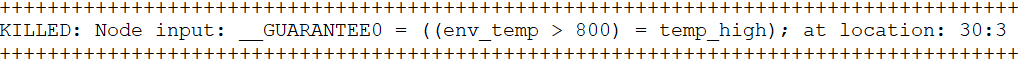
\includegraphics[scale=0.8]{images/guaranteesKilledSensor.PNG}
	\end{center}
	%\vspace{-1.5em}
	\caption{Temperature Subsystem Guarantee Killed by Equation Remover}
	\label{fig:guaranteesKilledSensor}
\end{figure}

After finding these results, we then defined a fault on the output governed by this guarantee and ran the minimal cut set generation on the fault model. As expected, this fault was in the minimal cut sets. While this example is sufficiently simple to illustrate the point, in complex models there can be multiple guarantees for a single component, many different components in a subsystem all of which are connected in various ways. It is obvious to anyone looking at the sensor subsystem model that this particular fault will violate the property. To this end, we turned our attention to a larger model: the Wheel Brake System as described in Section~\ref{chap:wbs}. At the time of this analysis, there were 33 fault nodes and 141 fault instances defined for 30 component types and 169 component instances throughout the extended system model. The total number of supporting guarantees within the nominal model was 246. We ran this analysis to see if there were other faults that may have been overlooked during the development of the WBS model. 

A guarantee on the hydraulic fuse component of the wheel brake subsystem was presented in a single layer mutation analysis as shown in Figure~\ref{fig:wheelBrakeGuaranteeKilled}. 

\begin{figure}[h]
	\begin{center}
		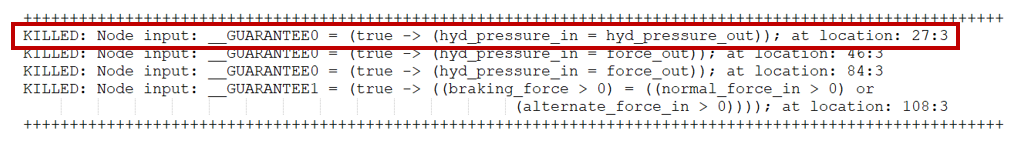
\includegraphics[scale=0.8]{images/wheelBrakeGuaranteesKilled.PNG}
	\end{center}
	%\vspace{-1.5em}
	\caption{Hydraulic Fuse Guarantee Killed by Equation Remover}
	\label{fig:wheelBrakeGuaranteeKilled}
\end{figure}

The guarantee presented governs the output of a hydraulic fuse attached to the wheel brake subsystem in the WBS. The guarantee states that the hydraulic pressure in is equal to the output. A stuck closed fault was defined on this fuse and minimal cut sets were generated for the WBS with cardinality restriction at one. Since this guarantee is a \mustcov\ element of the program, it should be the case that the fault is a single point of failure. The expected results are seen in the minimal cut sets as shown in Figure~\ref{fig:cutSetsWheelBrake}; the violation of the property occurs when this fault is present. 

\begin{figure}[h]
	\begin{center}
		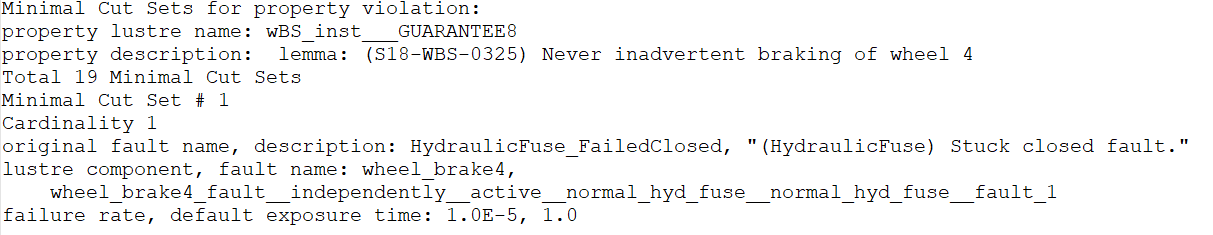
\includegraphics[scale=0.7]{images/cutSetsWheelBrake.PNG}
	\end{center}
	%\vspace{-1.5em}
	\caption{Hydraulic Fuse Fault in Minimal Cut Sets}
	\label{fig:cutSetsWheelBrake}
\end{figure}

Performing a kind of mutation analysis could be beneficial during the fault modeling process to catch things that may be missed during the fault definition process. The initial foray into mutation testing results show that this has potential for integration into the safety annex. It was also clear that a better presentation of the results was needed for large models. In the case of the WBS mutation analysis, over 240 guarantees were given as candidates for faults -- many of which already had faults associated with them. By integrating this feature into the fault analysis, these guarantees could be pruned from the output and save the user from pouring through potentially hundreds of guarantees as well as improve mutation engine time by eliminating the fault-associated guarantees from the analysis. Likewise, in the safety annex it is possible to generate the Lustre program if desired, but the common user will not reference the location of a guarantee this way. The location feature would need to be integrated into the safety annex and provide a link to the guarantee within the component AADL file.

\subsection{Node Inputs and Mutation Testing}
The equation remover mutation also iterates through Lustre node inputs and performs the mutation one input at a time. The node inputs in the Lustre model correspond to the inputs and outputs of an AADL component as shown in Figure~\ref{fig:nodeInputsLustre}. 

\begin{figure}[h]
	\begin{center}
		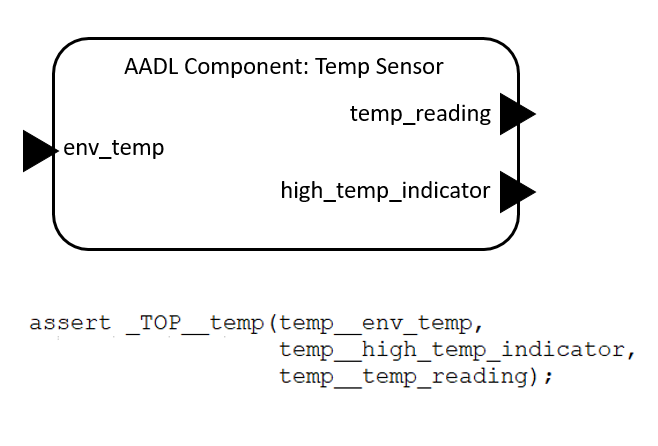
\includegraphics[scale=0.8]{images/nodeInputsLustre.PNG}
	\end{center}
	%\vspace{-1.5em}
	\caption{An AADL Component and Lustre Node Inputs}
	\label{fig:nodeInputsLustre}
\end{figure}

Given that the equation remover algorithm can perform this operation over node inputs, we can also gather information about critical outputs of components. Performing a similar extention to the equation remover algorithm, we collected all node input mutations that are killed and present them to the user. As an example, we show in Figure~\ref{fig:nodeInputsKilled} the analysis results on the nominal temperature subsystem example. 

\begin{figure}[h]
	\begin{center}
		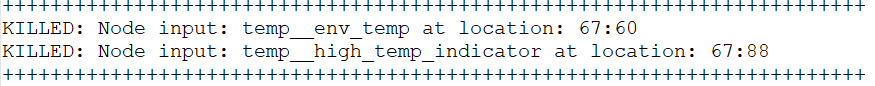
\includegraphics[scale=0.6]{images/nodeInputsKilled.PNG}
	\end{center}
	%\vspace{-1.5em}
	\caption{Temperature Node Inputs Killed by Equation Remover}
	\label{fig:nodeInputsKilled}
\end{figure}

Given that there exists an assumption on the temperature sensor input, we focus on the output. The only killed output was that of the high temperature indication, which tells us to prove the guarantee $\mathit{env\_temp} > 8 \iff \mathit{temp\_high}$, the output of this node is of utmost importance. Not surprisingly, when attaching a fault to this output, we get this fault in the minimal cut set for the top level property. 

As in the case with application of mutation testing on guarantees, node inputs also will require integration into the safety annex in order to filter out node inputs that have already been accounted for with faults in the extended system model. In large systems, this analysis is scalable and shows itself to be informative, but the outputs are unwieldy and large. Further work to rectify this would be required before use in large systems. 

The investigations into mutation testing applied to fault analysis were implemented in JKind and can be found at \url{https://github.com/dkstewart/jkind} on the {\em fault\_analysis\_mutations} branch.


\section{Preprocessing Improvements}
The preprocessing that must be done to generate minimal cut sets is not trivial. All minimal inductive validity cores must be produced which is as hard as model checking~\cite{GhassabaniGW16}. If all MIVCs are found, then these sets must be transformed into minimal correction sets through a minimal hitting set algorithm. Finding the hitting sets, or {\em set cover} is an NP-Complete problem itself in terms of cardinality alone~\cite{gainer2017minimal,murakami2013efficient}.%, but irreducibility is a weaker requirement and thus can be performed in polynomial time~\cite{liffiton2005finding}. While this is no longer NP-hard, the possible number of MIVCs may be large and thus the computation impractical. 
We performed extensive research into hitting set algorithms and implemented an open source option that performed well on benchmark testing~\cite{}, but nevertheless, these preprocessing steps could be fraught with peril when models become quite large and complex. We believe that a more direct approach to computing the minimal correction sets (MCSs) could be beneficial and is possible to implement as an additional JKind engine. This would eliminate the need to compute MIVCs and avoid the hitting set algorithm altogether. 

Liffiton et al.~\cite{liffiton2016fast} considered the enumeration of MCSs and MUSs as an exploration of the power set of all subclauses in a formula. The subsets form a lattice through subset relations and this lattice can be explored in clever ways in order to enumerate these related sets. A \texttt{map} is a boolean function used to encode the explored portions of the lattice. The entire lattice can be split into two regions based on the feasibility of the subset: these are the {\em maximally satisfiable subsets} (MSS) and the {\em minimally unsatisfiable subsets} (MUS). A maximally satisfiable subset is the complement of a MCS with respect to the constraint system; more formally, an MSS $M$ of a constraint system $C$ is a subset $M\subseteq C$ such that $M$ is satisfiable and $\forall c \in C \setminus M$ : $M \cup \{c\}$ is unsatisfiable. A full enumeration of the MSSs (also called the Max-SAT problem) will easily provide the full enumeration of the MCSs by taking the complement in $C$. 

The lattice structure ensures that any subset of a maximally satisfiable set is still satisfiable; thus, as subsets are explored, large portions of the map are eliminated from consideration. The CAMUS algorithm presented by Liffiton et al.~\cite{liffiton2005finding} uses the hitting set duality between MCS and MUS to produce MUSs by first computing MSSs, finding the complements (MCSs), and then producing the hitting sets (MUSs). It computes MCSs with what can be considered a top-down search through the power set, searching a level (subsets of a particular size) for satisfiable subsets that are not subsumed by some larger satisfiable subset found in a higher level. Whenever an MSS is found, all subsets are blocked from the \texttt{map} and the search moves on to the next level of the power set. The algorithms presented for this SAT-solver based enumeration of MUSs are (1) find all MCSs, and (2) compute MUSs. Related research has recently expanded upon the former algorithm used to enumerate MCSs by employing a correction set rotation method and simultaneously implementing the strengthening and relaxing methods described in the CAMUS algorithm~\cite{narodytska2018core}.  

We believe that these algorithms can be adjusted for SMT solvers and infinite state transition systems appropriately and then implemented in JKind. This will allow for a direct computation of MCSs and avoid the two preprocessing steps (MIVC generation and MHS generation) as outlined in this dissertation. 




%We also believe that the total verification time can be improved by focusing on preprocessing steps. In the minimal cut set generation preprocessing, the MIVCs are collected, the hitting sets computed, and then our algorithm is run based on the minimal correction sets found in the previous two steps. By eliminating the need for MIVCs altogether and directly computing the minimal correction sets from the Lustre program, we believe this could improve computation time. 
